\documentclass[12pt,a4paper,frenchb]{article}

\input{../../commons.tex.inc}

\makeatletter

\renewcommand{\maketitle}%
{\framebox{%
    \begin{minipage}{1.0\linewidth}%
      \begin{center}%
        \Large \@title ~-- \@author \\%
        \@date%
      \end{center}%
    \end{minipage}}%
  \normalsize%
  %\vspace{1cm}%
}

\makeatother

\setlength{\parsep}{0pt}
\setlength{\parskip}{5pt}
\setlength{\parindent}{0pt}
\setlength{\itemsep}{7pt}

\everymath{\displaystyle\everymath{}}


\title{Limites de fonctions}
\author{Terminale S}
\date{octobre 2017}

\begin{document}

\maketitle

\section{Limite à l'infini}

\subsection{Limite finie}

Comme vu dans les activités 1 et 2 pages 52 53, on étend la définition
de la limite vue sur les suites aux fonctions, au moins dans un premier
temps sur les fonctions monotones sur tous les intervalles de la forme
$\intv[r]*{A}{+\infty}$, avec $A > 0$.

\framebox{
  \begin{minipage}{0.99\linewidth}
    \begin{definition}
    \end{definition}
    \vspace{4cm}
  \end{minipage}
}

De façon générale, si la fonction et monotone, $\lim_{x\to+\infty} f(x)
= \lim_{n\to\infty}f(n)$.

\begin{center}
  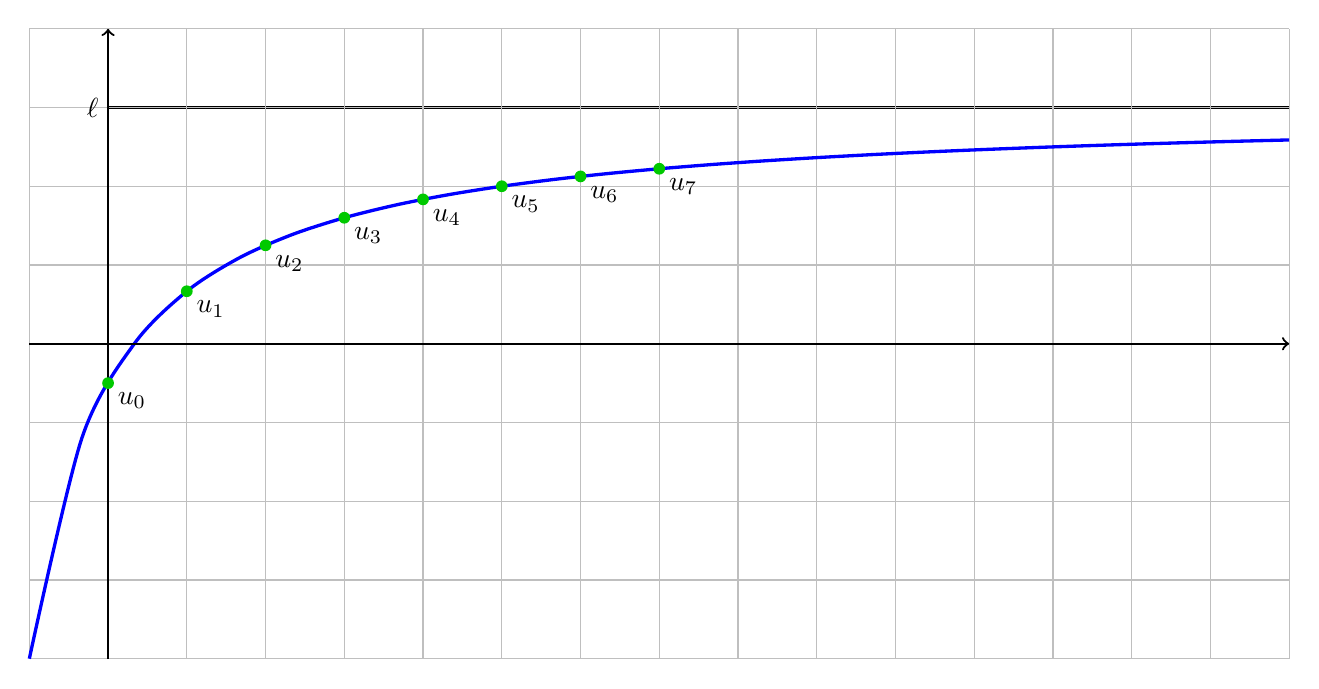
\begin{tikzpicture}
    \def\A{12.5}
    \draw [black, very thick] (0,3) -- (15,3) ;
    \draw [thin, lightgray] (-1,-4) grid [step=1] (15,4) ;
    \draw [very thick, blue] plot [domain = -1:15,smooth]
    (\x,{(3*\x-1)/(\x+2)}) ;
    \draw [thick,->] (-1,0) -- (15,0) ;
    \draw [thick,->] (0,-4) -- (0,4) ;
    \foreach \x in {0,...,7} { \draw (\x,{(3*\x-1)/(\x+2)}) node
      [circle, fill, green!79!black, inner sep=1.5pt] {} ;
      \draw (\x,{(3*\x-1)/(\x+2)}) node [below right] {$u_{\x}$ } ;
    }
    \draw (0,3) node [left] {$\ell$} ;
  \end{tikzpicture}
\end{center}

Dans ce cas, on peut interpréter graphiquement le résultat précédent :

\framebox{
  \begin{minipage}{0.99\linewidth}
    Soit $f$ une fonction admettant $\ell$ pour limite en $\pm\infty$.

    La droite d'équation \vspace{9mm}\hspace{2cm} est une
    \vspace{9mm}\hspace{6cm} à la courbe représentative de la fonction
    $\mathscr{C}_f$.
  \end{minipage}
}

Attention toute fois à éviter les raisonnements trop hâtifs !
\begin{exemple}
  Soit $f$ la fonction définie par $\forall x\in\R, f(x) = \frac{\cos(2n\pi x)
  +1 }{2}$. On a clairement $f(n) = 1 \forall n \in\N$ et donc
  $\lim_{n\to+\infty}f(n) = 1$ et pourtant $\lim_{x\to\infty} \neq 1$ et
  même n'a pas de limite.
  \begin{preuve}
    Il s'agit de démontrer que $\forall \ell \in \intv[c]*{0}{1},\exists
    \varepsilon > 0,\ \exists A,\ x > A \implies \vabs{x - \ell} >
    \varepsilon$.

    Soit $\ell$ dans $\intv*{0}{1}$, (par exemple 1) pour $\varepsilon =
    \np{0.1}$, pour $x = \np{1254},\ \vabs{x - 1} < \varepsilon$, mais
    pour $x = A + \frac12,\ x\not\in \intv[o]*{\ell - \varepsilon}{\ell +
    \varepsilon}$
  \end{preuve}
\end{exemple}

Par symétrie verticale selon l'axe des ordonnées, on peut appliquer le
même type de raisonnement dans le cas où $x$ tend vers $-\infty$.


\subsection{Limite infinie}

Pour les fonctions, on parle aussi bien de limite infinie ou de
divergence vers $\pm\infty$.

\framebox{
  \begin{minipage}{0.99\linewidth}
    \begin{definition}
    \end{definition}
    \vspace{4cm}
  \end{minipage}
}

On peut faire la même remarque dans le cas précédent !

On peut parfois interpréter ce cas graphiquement :

\begin{minipage}{0.99\linewidth}
  Soit $f$ une fonction admettant $+\infty$ pour limite en $+\infty$.

  S'il existe une droite d'équation \hspace{2cm} telle que
  $\lim_{x\to+\infty}f(x) - y = 0$, on dit alors que cette droite est
  une \vspace{9mm}\hspace{6cm} à la courbe représentative de la fonction
  $\mathscr{C}_f$.
\end{minipage}

\subsection{Limite en un point}
Le cas qui nous intéresse le plus est celui de la limite infinie en un
point.

\framebox{
  \begin{minipage}{0.99\linewidth}
    \begin{definition}
    \end{definition}
    \vspace{4cm}
  \end{minipage}
}

L'exemple type et connu est celui de la fonction homographique de «base»
: la fonction inverse $x\mapsto \frac1x$

\begin{center}
  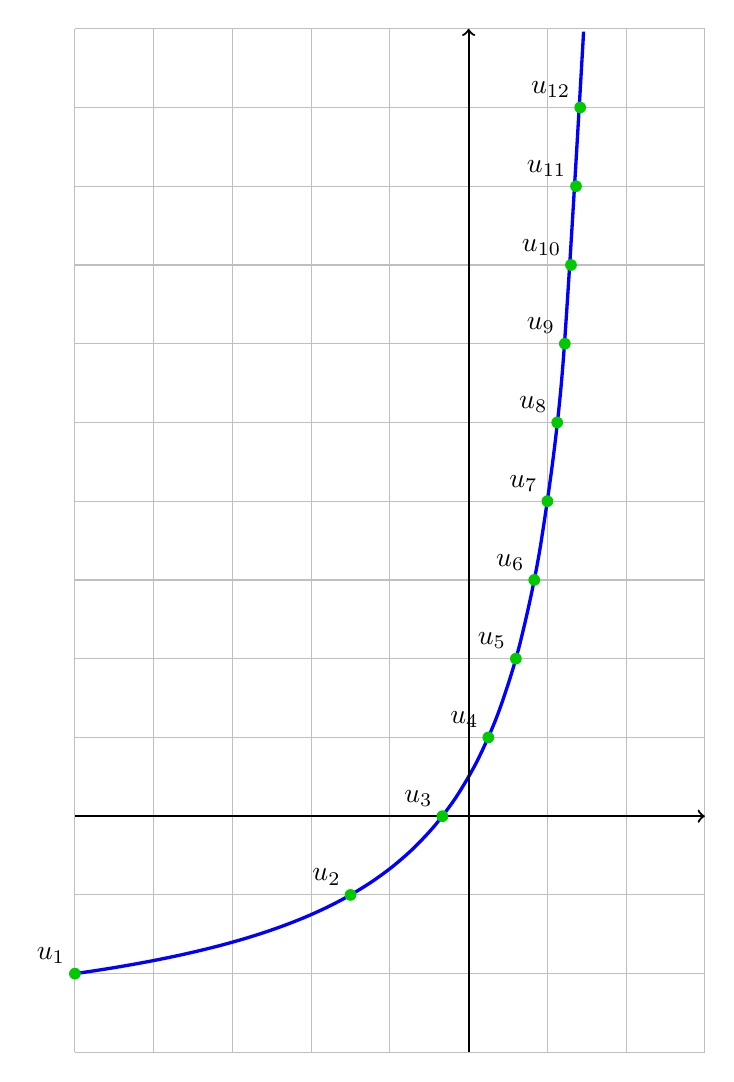
\begin{tikzpicture}
    \def\a{2}
    \def\A{7}
    \def\e{0.7}

    \draw [thin, lightgray] (-5,-3) grid [step=1] (3,10) ;
    \draw [very thick, blue] plot [domain = -1.46:5,smooth]
    (-\x,{-(3*\x-1)/(\x+2)}) ;
    \draw [thick,->] (-5,0) -- (3,0) ;
    \draw [thick,->] (0,-3) -- (0,10) ;
    \foreach \x in {1,...,12} { \draw (2-7/\x,{-(3*(-2+7/\x)-1)/((-2+7/\x)+2)}) node
      [circle, fill, green!79!black, inner sep=1.5pt] {} ;
      \draw (-7/\x+2,{-(3*(7/\x-2)-1)/((7/\x-2)+2)}) node [above left]
      {$u_{\x}$ } ;
    }

  \end{tikzpicture}
\end{center}

\framebox{
  \begin{minipage}{0.99\linewidth}
    Soit $f$ une fonction admettant $\pm\infty$ pour limite en $a$.

    La droite d'équation \vspace{9mm}\hspace{2cm} est une
    \vspace{9mm}\hspace{6cm} à la courbe représentative de la fonction
    $\mathscr{C}_f$.
  \end{minipage}
}

\section{Opérations sur les limites}

\subsection{Limites en $\pm\infty$}

On peut ici reprendre le cours sur les suites et le relire en remplaçant
$u_n$ par $f(x)$, aussi bien pour les théorèmes de comparaisons que pour
les opérations.

\subsection{Limites finies}

Soient $f$ et $g$ deux fonctions, définies respectivement sur
$\mathcal{D}_f$ et $\mathcal{D}_g$, avec $f(\mathcal{D}_f)\subset
\mathcal{D}_g$.

On suppose que $\lim_{x\to a}f(x) = b$, avec $a\in\mathcal{D}_f$ et
$b\in\mathcal{D}_g$.

Alors $\lim_{x\to a}g(f(x))$ existe et vaut $g(b)$ ou la limite de $g$
en $b$.

\begin{remarque}
  Avec les hypothèses ci-dessus pour le domaine de définition et le
  domain image, la fonction $x\mapsto g(f(x))$ se note $(g\circ f)(x)$
  ou plus simplement $g\circ f(x)$
\end{remarque}

\begin{exemple}
  $\lim_{x\to+\infty}\sin\frac{2}{\sqrt{x-2}}$
\end{exemple}

\end{document}
